
\section{Linear Regression Models}
We start from the \textit{univariate linear regression}, i.e., each output consists of a single value while the input is a vector of values.

\subsection{Univariate linear regression}
Univariate means single output, i.e, $y$ is a number. The basic form is 
\begin{align}
f(X) = \beta_0 + \sum_{j-1}^p X_j \beta_j
\end{align}

The most popular estimation method for a linear model is the least square:
\begin{align}
RSS(\beta) = \sum_{i=1}^{p}  \left( y_i - f(x_i) \right)^2 = \left(\bm{y} - \bm{X}\beta\right)^T \left(\bm{y} - \bm{X}\beta\right)
\end{align}

where $\bm{X}$ is a $N \times (p+1)$ matrix with each row being an input vector, $\bm{y}$ a $N$ vector (we must have $N$ input-output pairs, in this case the output is considered mono-dimensional).

By minimizing we get:

\begin{align}
\hat{\beta} = \left( \X^T \X\right)^{-1} \X^TY
\label{OLSRegression}
\end{align}
Geometrically we are projecting $y$ onto the hyperplane spanned by $X$ and the projections is referred to as $\hat{y}$:

\begin{align}
\hat{y} =\X \left( \X^T \X\right)^{-1} \X^T Y = H Y
\end{align}
where $H$ is called the \textit{hat} matrix.


%%%%%%%%%%%%%
\subsection{Equivalence of Ordinary least squares and maximum likelihood}
We are using an additive model, assuming a Gaussian white noise:
\begin{align}
y = \beta^T \x + \epsilon \\
\epsilon \sim \CMcal{N}(0,\sigma^2)
\end{align}
Adding a constant to a Gaussian random variable is equivalent to another Gaussian random variable with the mean shifted:
\begin{equation}
Pr(y) \sim \CMcal{N}(\beta^T \x ,\sigma^2)
\end{equation}
Considering the matrix $\X$ and the output vector $\y$ representing the training set, used to estimate the coefficients, we have:
\begin{equation}
Pr(\y|\X, \beta, \sigma^2)  = \prod_{i=1}^N Pr(y_i|\x, \beta, \sigma^2) =  \prod_{i=1}^N \CMcal{N}(\beta^T \x ,\sigma^2)
\end{equation}
where we have assumed each observation is independent. A product of univariate Gaussian can be rewritten as a multivariate Gaussian:
\begin{equation}
\label{multiGauss}
\begin{aligned}
 &Pr(\y|\X, \beta, \sigma^2)  = \prod_{i=1}^N \CMcal{N}(\beta^T \x ,\sigma^2) =  \prod_{i=1}^N \frac{1}{(2\pi)^{\frac{1}{2}}\sigma}e^{-\frac{\left(y_i-\beta^T\x_i\right)^2} {2\sigma^2}}= \\
 &= \frac{1}{(2\pi)^{\frac{p}{2}}\sigma}\prod_{i=1}^N e^{-\sum_{i=1}^N \frac{\left(y_i-\beta^T\x_i\right)^2} {2\sigma^2}} = \\
 &=  \frac{1}{(2\pi)^{\frac{p}{2}}\sigma|\mathbf{I}|}e^{-\frac{1}{2}\left(\y-\beta^T\X\right)^T\left(\sigma^2 \mathbf{I}\right)^{-1}\left(\y-\beta^T\X\right)} = \CMcal{N}(\beta^T \X ,\sigma^2\mathbf{I}) 
\end{aligned}
\end{equation}
If the variables are not independent the more general form is:
\begin{equation}
\CMcal{N}(\beta^T \X ,\mathbf{\Sigma}) =\frac{1}{(2\pi)^{\frac{p}{2}}|\Sigma|^\frac{1}{2}}e^{-\frac{1}{2}\left(\y-\beta^T\X\right)^T\Sigma^{-1}\left(\y-\beta^T\X\right)}
\end{equation}

%%%%%%%%
\paragraph{Definition of likelihood}
The quantity $Pr(y|\x, \beta, \sigma^2)$ is called \textbf{likelihood} and tell us how much it is likely the outcome $y_i$ in the dataset given the input $\x$ and the parameters.

A different approach to find a model that fits the data is to maximize the \textit{likelihood} of the whole dataset:
\begin{equation}
L = Pr(\y|\X, \beta, \sigma^2)  = \frac{1}{(2\pi)^{\frac{p}{2}}|\Sigma|^\frac{1}{2}}e^{-\frac{1}{2}\left(\y-\beta^T\X\right)^T\Sigma^{-1}\left(\y-\beta^T\X\right)}
\end{equation}

Actually maximizing the likelihood is equivalent to maximizing its logarithmic, the \textit{log-likelihood}:
\begin{equation}
\begin{aligned}
&\log L = \sum_{i=1}^N \log\left[\frac{1}{(2\pi)^{\frac{1}{2}}\sigma}e^{-\frac{\left(\y_i-\beta^t \x_i\right)^2} {2\sigma^2}}\right]\\
&=\sum_{i=1}^N -\frac{1}{2}\log2\pi -\log \sigma -\frac{\left(y_i-\beta^T\x_i\right)^2} {2\sigma^2} =\\
&= -\frac{1}{2}\log2\pi -\log \sigma -\frac{1}{2\sigma^2} \sum_{i=1}^N\left(y_i-\beta^T\x_i\right)^2
\end{aligned}
\end{equation}
As already done for OLS, taking the derivative w.r.t. $\beta$ and setting it to $0$:
\begin{equation}
\begin{aligned}
&\frac{\partial \log L}{\partial \beta} = -\frac{1}{2\sigma^2} \left(-2\right) \left(\y_i-\beta^T\x_i\right) = 0 \\
&\Rightarrow \left(\y-\beta^T\X \right)= 0 \Rightarrow \beta = \HM \y
\end{aligned}
\end{equation}

This is the same solution of the OLS: the two models are equivalent.

\textbf{The two models are equivalent assuming a normal distribution}.

\subsection{Expectation of the parameter estimation: unbiased estimator}
Computing the expectation of $\hat{\beta}$:
\begin{equation}
\begin{aligned}
&\E_{Pr(\y|\X,\beta, \sigma^2)}\left[ \hbe\right]= \sum \hbe Pr(\y|X, \beta, \sigma^2) =\\
&= \HM \sum \y Pr(\y |X, \beta, \sigma^2)  = \\
&=\HM \E_{Pr(\y | \X,\beta, \sigma^2)} \left[ \y\right] = \\
&= \HM \X \beta = \beta
\end{aligned}
\end{equation}

This is an \textbf{unbiased estimator}.

Now let us calculate the covariance matrix:
\begin{equation}
\begin{aligned}
&\Cov \left[\hb \right] = \\
&=\E_{Pr(\y|\X,\beta, \sigma^2)}\left[ \left( \hb -\E_{Pr(\y|\X,\beta, \sigma^2)}\left[ \beta\right] \right) \left( \hb -\E_{Pr(\y|\X,\beta, \sigma^2)}\left[ \beta\right] \right)^T\right] = \\
&=\E_{Pr(\y|\X,\beta, \sigma^2)}\left[ \left( \hb - \beta \right) \left( \hb - \beta \right)^T\right] =\\
&=\E_{Pr(\y|\X,\beta, \sigma^2)}\left[ \hb\hb^T\right] -\beta\beta^T\end{aligned}
\end{equation}
and
\begin{equation}
\begin{aligned}
&\E_{Pr(\y|\X,\beta, \sigma^2)}\left[ \hb\hb^T\right] = \\
&=\E_{Pr(\y|\X,\beta, \sigma^2)} \left[ \left( \HM \y\right)\left( \HM \y\right)^T\right] = \\
& = \HM\E_{Pr(\y|\X,\beta, \sigma^2)} \left[   \y  \y^T\right] \X \inv
\end{aligned}
\end{equation}
and recalling from \autoref{multiGauss} $Pr(\y) \sim \CMcal{N}(\beta^T \X ,\sigma^2 \mathbf{I})$
\begin{equation}
\begin{aligned}
&\Cov\left[ \y\right]=\sigma^2 \mathbf{I} =\\
&=\E_{Pr(\y|\X,\beta, \sigma^2)}\left[ \y\y^T\right]  - \E_{Pr(\y|\X,\beta, \sigma^2)}\left[ \y\right]\E_{Pr(\y|\X,\beta, \sigma^2)}\left[ \y^T\right]\\
\end{aligned}
\end{equation}

Rearranging
\begin{equation}
\begin{aligned}
&\Rightarrow \E_{Pr(\y|\X,\beta, \sigma^2)}\left[ \y\y^T\right] = \sigma^2 \mathbf{I} +\E_{Pr(\y|\X,\beta, \sigma^2)}\left[ \y\right]\E_{Pr(\y|\X,\beta, \sigma^2)}\left[ \y^T\right] =\\
&=\sigma^2 \mathbf{I} +\E_{Pr(\y|\X,\beta, \sigma^2)}\left[ \X\beta\right]\E_{Pr(\y|\X,\beta, \sigma^2)}\left[ \beta^T\X^T\right] =\\
&= \sigma^2 \mathbf{I} +\X\beta \beta^T\X^T
\end{aligned}
\end{equation}

Substituting:

\begin{equation}
\begin{aligned}
&\E_{Pr(\y|\X,\beta, \sigma^2)}\left[ \hb\hb^T\right] = \HM \left(\sigma^2 \mathbf{I} +\X\beta \beta^T\X^T\right)X \inv   = \\
 &=\sigma^2 \inv 
\end{aligned}
\end{equation}

and finally variance-covariance matrix of the least square parameters is 
\begin{equation}
\begin{aligned}
&\Cov\left[ \hb\right]=  \inv  \sigma^2
\end{aligned}
\end{equation}
 
\begin{align}
Var(\hat{\beta}) = (\X^T\X)^{-1} \sigma^2
\end{align}

\subsection{Noise variance estimation}
We can find an estimation of the noise variance from the maximum likelihood model using the same procedure used to find the parameters, i.e., taking the derivative and equating it to $0$:
\begin{equation}
\begin{aligned}
\label{varErr}
&\frac{\partial \log L}{\partial \sigma} = \sum_{i=1}^N-\frac{1}{\sigma} +\frac{1}{\sigma^3} \left(y_i - \x_i^T\beta\right)^2 = 0 \Rightarrow \frac{N}{\sigma} +\frac{1}{\sigma^3}  \sum_{i=1}^N\left(y_i - \x^T\beta\right)^2 = 0\\
&\Rightarrow \hat{\sigma^2} = \frac{1}{N}\sum_{i=1}^N\left(y_i - \x_i^T\beta\right)^2 
\end{aligned}
\end{equation}
This can be re-expressed as
\begin{equation}
\begin{aligned}
&\Rightarrow \hat{\sigma^2} = \frac{1}{N}\sum_{i=1}^N\left(y_i - \x^T\hb\right)^2  = \frac{1}{N}\sum_{i=1}^N\left(y_i - \x_i^T\HM\y\right)^2 = \\
&= \frac{1}{N}\left(\y - \X\HM\y\right)^T\left(\y - \X\HM\y\right) = \\
&=\y^T\y  - 2 \y^T  \X\HM\y + \y^T \X \cancel{\inv} \cancel{\X^T \X}\HM\y = \\
&=\y^T\y  - \y^T  \X\HM\y  = \left(\y^T\y - \y^T\X\hb \right)
\end{aligned}
\end{equation}

Taking the expectation w.r.t. $Pr(\y|\X,\beta, \sigma^2)$:
\begin{equation}
\begin{aligned}
&\E_{Pr(\y|\X,\beta, \sigma^2)} \left[\hs\right] = \frac{1}{N}\E_{Pr(\y|\X,\beta, \sigma^2)} \left[\y^T\y - \y^T\X\hb \right] =\\
&=\frac{1}{N}\E_{Pr(\y|\X,\beta, \sigma^2)} \left[\y^T\y \right] - \frac{1}{N}\E_{Pr(\y|\X,\beta, \sigma^2)} \left[\y^T\X\HM \y \right] 
\end{aligned}
\end{equation}

Suppose $\mathbf{t} \sim  \CMcal{N}\left(\mathbf{\mu}, \mathbf{\Sigma} \right)$, then $\E_{p(\mathbf{t})} \left( \mathbf{t^TAt}\right)= \Tr(\mathbf{A\Sigma})+\mathbf{\mu^TA\mu}$ with $\mu = \X\beta$

\begin{equation}
\begin{aligned}
&\E_{Pr(\y|\X,\beta, \sigma^2)} \left[\hs\right] =\frac{1}{N}\E_{Pr(\y|\X,\beta, \sigma^2)} \left[\y^T\y \right] +\\
&- \frac{1}{N}\E_{Pr(\y|\X,\beta, \sigma^2)} \left[\y^T\X\HM \y \right]  = \\
&= \frac{1}{N}\E_{Pr(\y|\X,\beta, \sigma^2)} \left[\y^T\mathbf{I}_N\y \right] +\\
&- \frac{1}{N}\E_{Pr(\y|\X,\beta, \sigma^2)} \left[\y^T\X\HM \y \right]  = \\
&=\frac{1}{N}\left(\Tr\left(\sigma^2\mathbf{I}_N\right) +\beta^T\X^T\X\beta \right) + \\
&- \frac{1}{N}\left(\Tr\left[\sigma^2\X\HM\right] +\beta^T\X^T\X\HM\X\beta  \right) =\\
&= \frac{1}{N}\left(N\sigma^2 +\beta^T\X^T\X\beta \right) - \frac{1}{N}\left(\sigma^2\Tr\left[\X\HM\right] +\beta^T\X^T\X\beta  \right) =\\
&= \sigma^2 +\cancel{\frac{1}{N}\beta^T\X^T\X\beta} -\frac{\sigma^2}{N}\Tr\left[\X\HM\right] \cancel{-\frac{1}{N}\beta^T\X^TX\beta} = \\
&=\sigma^2 -\frac{\sigma^2}{N}\Tr\left[\HM\X\right] = \sigma^2 -\frac{\sigma^2}{N}\Tr\left[\mathbf{I}_p\right]  \\
&\Rightarrow \E_{Pr(\y|\X,\beta, \sigma^2)} \left[\hs\right] = \sigma^2 \left( 1 - \frac{p}{N}\right)
\end{aligned}
\end{equation}
where lastly we have used the product property of the trace (see \autoref{trace}).

Normally $p<N$ hence the estimate of the variance is smaller than the true variance, so this estimator is \textbf{biased}. The estimate gets closer to the real value when $p/N$ is small, i.e., assuming $p$ is fixed, increasing the samples used. 

This result might be strange. First of all notice from \autoref{varErr} that the closer the model gets to the data, the smaller $\hs$. By definition the parameter estimates are the ones that minimise the noise and hence $\hs$. As a consequence, when using the true parameters we would get equal or higher variance.

To estimate the true variance we can use the following formula:
\begin{align}
\hat{\sigma}^2 = \frac{1}{N-p-1}\sum_{i=1}^{N}(y_i-\hat{y}_i)^2
\end{align}
$N-p-1$ makes this estimation unbiased i.e., $\frac{1}{N-p-1}\E[\hat{\sigma}^2] =\sigma^2$.

\subsection{Interpretation of covariance}
Consider a covariance matrix of size $2\times 2$ for a two parameter model (i.e., a line on the plane) and suppose the first diagonal element, corresponding to the variable $\hb_0$ is much bigger than the second one corresponding to $\hb_1$. This means that we can change $\hb_0$ a little without affecting too much the model. On the contrary if the variance is small, small changes will affect significantly the model. Sometimes this happens when one variable has a much higher absolute value.

If the values on the off-diagonals are negative, then when increasing one coefficient i.e., $\hb_0$, the other must be decreased to have the line to pass as close as possible to all points. For example in $2D$, increasing $\hb_0$ reduces the coefficient value: if it is positive, the line will be "more horizontal", if negative it becomes steeper, "more vertical".
\subsection{Z-score}
Let us assume data were really generated by a linear model but were corrupted by Gaussian noise with $0$ mean and variance $\sigma^2$:

\begin{align}
Y = \beta_0 +\sum_i^p \beta_i X_i + \epsilon
\end{align} 
where $\epsilon \sim \CMcal{N}(0,\sigma^2)$.
The estimated parameters will still be a normal distribution:

\begin{align}
\label{parameterVar}
\hat{\beta} \sim \CMcal{N}(\beta,  (\X^T\X)^{-1} \sigma^2)
\end{align}

\begin{definition}{\textbf{Z-score}}
A Z-score, is a numerical and statistical measurement of a value's relationship to the mean (average) of a group of values, measured in terms of standard deviations from the mean. If a Z-score is 0, it indicates that the data point's score is identical to the mean score. A Z-score of 1.0 would indicate a value that is one standard deviation from the mean. Z-scores may be positive or negative, with a positive value indicating the score is above the mean and a negative score indicating it is below the mean. Z-scores are measures of an observation's variability

\begin{align}
z_j=\frac{x - \mu}{\sigma}
\end{align}

In machine learning the z-value is generally intended as the regression coefficient divided by its standard error. It is also sometimes called the z-statistic. If the z-value is too big in magnitude (i.e., either too positive or too negative), it indicates that the corresponding true regression coefficient is not $0$ and the corresponding X-variable matters. A good rule of thumb is to use a cut-off value of $2$ which approximately corresponds to a two-sided hypothesis test with a significance level of $\alpha=0.05$.

Z-values are computed as the test statistic for the hypothesis test that the true corresponding regression coefficient $\beta_j$ is $0$. In hypothesis testing, one assumes the null hypothesis is true, and then see if data provide evidence against it. So in this case, $\beta$ is assumed to be  $0$. That is, the expectation of the fitted regression coefficient $\hat{\beta}$ is assumed to be $0$:

\begin{align}
z_j =\frac{\hat{\beta}_j}{\hat{\sigma} \sqrt{v_j}}
\end{align}
where the denominator is the standard deviation (root square of the variance) of the parameter (from \autoref{parameterVar}) with $v_j$ being the diagonal element of $(X^TX)^{-1}$.
\end{definition}

Being the parameters normally distributed by assumption, the standard error tells you how far on average sample parameters tend to deviate from the mean population parameter, i.e., from the true parameter $\be$.

\begin{theorem}[\textbf{The Gauss-Markov theorem}]
Among all linear unbiased estimators, the least square estimates of the parameters are the ones having smallest variance and consequently from \autoref{biasVar} is the one with the smallest mean squared error (the bias-squared term for unbiased estimator is by definition $0$).
\begin{proof}
Let $\hat{\beta} = Cy$ be another linear estimator of $\beta$ with $C = (X^TX)^{-1}X^T+D$
\begin{align}
&\E\left[ \hat{\beta} \right] = \E\left[ Cy \right] = \E\left[\left(\left(X^TX\right)^{-1}X^T+D\right) \left( X\beta+\epsilon\right)\right] =\\
& = \left(\left(X^TX\right)^{-1}X^T X\beta +DX\beta\right) +\cancel{\left(\left(X^TX\right)^{-1}X^T  +D\right) \E[\epsilon]}=\\
& = \left(\beta +DX\beta\right) = \left( I +DX\right) \beta\\
\end{align}
where $ \E[\epsilon] = 0$.

To be an unbiased estimator $DX = 0$, then

\begin{equation}
\begin{aligned}
\Var(\hat{\beta}) &= \Var(Cy) = C\Var(y) C^T = \sigma^2 CC^T = \\
&= \sigma^2 \left( \left(X^T X\right)^{-1}X^T +D \right)    \left( \left(X^T X\right)^{-1}X^T+D\right)^T =\\
&= \sigma^2 \left( \left(X^T X\right)^{-1}X^T +D \right)    \left( X \left(X^TX\right)^{-1} + D^T \right)  =\\
&= \sigma^2 (  \cancel{\left(X^TX\right)^{-1}}\cancel{X^T X}   \left(X^TX\right)^{-1} +  \left(X^T X\right)^{-1}X^TD^T                          +\\
&\quad + D X \left(X^TX\right)^{-1} +DD^T) =\\
&= \sigma^2 (  \cancel{\left(X^TX\right)^{-1}}\cancel{X^T X}   \left(X^TX\right)^{-1} +  \left(X^T X\right)^{-1}\left( DX \right)^T                          +\\
&\quad + D X \left(X^TX\right)^{-1} +DD^T) \\
DX=0 \\\Rightarrow \Var(\tilde{\beta}) &= \sigma^2 \left( \left(X^TX\right)^{-1} +  \cancel{\left(X^T X\right)^{-1}\left( DX \right)^T }  + \cancel{D X \left(X^TX\right)^{-1} }+DD^T\right) \\
\Var(\tilde{\beta}) &= \Var(\hat{\beta})  + \sigma^2DD^T
\end{aligned}
\end{equation}

\end{proof}
\end{theorem}
\subsection{Orthogonalization}
Normally inputs are not perpendicular but can be orthogonalized. The goal is to define a new orthogonal basis for the data. The procedure, named \textbf{Grand-Schmidt procedure} consists of building up a new matrix of our data starting from $\X$ matrix, whose columns are orthogonal. The new columns are obtained as linear combinations of the columns of $\X$, hence they span the same space. The procedure can be summarized in the following steps:
\begin{algorithm}[!ht]
initialize $z_0=x_0=\mathbf{1}$ where $\mathbf{1}$ is a vector of all ones\;
For $j=1,\cdots, p$ regress $x_j$ on $z_0,\cdots, z_{p-1}$ to produce the coefficients $\hat{\gamma}_{lj}= \frac{\langle z_l , x_j\rangle}{\langle z_\ell , z_\ell\rangle}$ for $l=0,\cdots, j-1$\;
Calculate the residual vectors as $z_j = x_j - \sum_{k=0}^{j-1} \hat{\gamma}_{kj}z_k$\;
Regress $\mathbf{y}$ on the residual $z_p$ to get the estimate $\hat{\beta}_p = \frac{\langle z_p, y\rangle}{\langle z_p , z_p\rangle}$
\end{algorithm}
The first row of $\Gamma$ is $(1, 0, 0,\cdots 0)$ because of the initialization of
$x_0, z_0$ as vectors of ones in the first step of the algorithm. From a mathematical point of view we are building orthogonal vectors that describe the same space of the one described by the column of $\X$. To start the orthogonalization procedure, we take the first column vector of $\X$ as it is, in other words, the first direction
remains the same and we are not rescaling the vector. At the second step, we take the second column vector of $\X$, we project it onto $z_0$ to get the coefficient $\Gamma_{1,0}$, and then we get the second direction orthogonal to the first one as the vectorial difference of the column of $\X$ and its projection.

When inputs are correlated, the residual will be close to zero generating instabilities in the coefficients $\hat{\beta}_j$ and the z-score will be small.

The algorithm in matrix form is
\begin{align*}
\mathbf{X = Z\Gamma}
\end{align*}
where $z_j$ are the column vectors of $Z$ and $\Gamma$ is upper triangular. Introducing the diagonal matrix $D$ with $j$-th diagonal element $D_{jj}=||z_j||$ we get:

\begin{equation}
\mathbf{X = ZD^{-1}D\Gamma = QR}
\end{equation}
where $Q$ is an orthogonal, $Q^TQ=I$, $ N\times(p+1)$ matrix and $R$ is a $(p+1)(p+1)$ upper triangular matrix. The $Q$ matrix contains an orthonormal basis spanning the same space spanned by $\X$. The $R$ matrix contains the coefficients that multiply the orthonormal basis to get back the original matrix $X$. Consider the first step of the orthogonalization procedure. It takes the first column of $\X$ and just rescales it to have norm $1$. So to get back the first column of vector just a coefficient is needed. Hence, the first column of $R$ is just a column of $0$s except the first term. Then the second column of $\X$ is projected onto $q_1$ to get the first multiplier: this is the first element of the second column of $R$.The residual is perpendicular to $q_1$ and can be used as second axis after normalization: the scale factor is the second element of the column of $R$, all the other elements will be $0$. That is why $R$ is upper triangular.

The least square solution becomes 
\begin{equation}
\begin{aligned}
\hat{\beta} &= R^{-1}Q^Ty\\
\hat{y} &= QQ^Ty
\end{aligned}
\end{equation}

\subsection{Multivariate output}
We can rewrite the equation in matrix form:

\begin{equation}
Y = XB + E
\end{equation}
where $Y$ is  a $N\times K$ matrix, $X$ is $N\times(p+1)$, $B$ is $(p+1)\times K$, $E$ has the same dimensions of $Y$.
The root squared error is 
\begin{equation}
\begin{aligned}
RSS(B) &= \sum_{k=1}^K\sum_{i=1}^N\left(y_{ik}-f(x_i)\right)^2 = tr \left[  \left( Y-XB\right)^T\left( Y-XB\right) \right]	\\
\Rightarrow B &= \left( X^TX\right)^{-1}X^TY
\end{aligned}
\end{equation}
Multiple outputs do not affect one another's least square estimates.

\subsection{Subset selection}
Least square estimates sometimes show low bias but high variance resulting in a non-satisfactory prediction accuracy. This can be improved by setting some coefficients to $0$ to sacrifice a little of bias to reduce significantly the variance.

Other times it is useful to reduce the input dimensionality for easiness of interpretation or for computation purposes.

\subsubsection{Best subset selection}
This algorithm finds for each $k \in {0,1,2,	\cdots p}$, the subset of size $k$ that gives the smallest residual sum of squares. Note that if a variable is in the best subset of size $m$, it might not be in the subsets of larger size (and of course neither in the smallest ones).

\subsubsection{Forward stepwise selection}
Searching for all the subsets is too computationally intensive (and infeasible for $p>40$). The \textit{forward stepwise} algorithm starts with the intercept and then sequentially adds to the model the predictor that most improves the fit. $QR$ decomposition can be exploited to choose the next candidate. Particularly, we start from the intercept so that the first normal vector, $q_1$ is derived from the column of $1$s by normalization. At each step we will have $q$ vector features that have already been used to form a partial basis $Q_q$ of size $n\times q$, and the remaining $p-q$ features that still must be exploited. For each remaining feature, calculate the residual:

\begin{equation}
r_k  = x_k - \left(x_k^T Q_qQ_q^T\right)^T = x_k - Q_qQ_q^Tx_k
\end{equation}
The possible orthonormal vector is the normalized residual, $\tilde{q}_{q+1}$. The column $x_k$ to be considered to form the new direction $q_{q+1}$ is the one for which the product $y^T \tilde{q}_{q+1}$ is maximized. From this best candidate and the matrix $Q_{q}$, we build the matrix $Q_{q+1}$:
\begin{equation}
Q_{q+1} = \left[Q_{q}, q_{q+1}\right]
\end{equation}
The $R$ matrix must be updated too: first a row of zeros is appended to the end. Then a column containing the coefficients is obtained by projection of the vector $x_k$ onto $Q_{q+1}$:

\begin{equation}
  R_{q+1} = 
  \left[ \begin{array}{ *{5}{c} }
    & & &\text{\Large{$|$}}  &\\
    & &&\text{\Large{$|$}} &  \\
    \multicolumn{3}{c}
      {\raisebox{\dimexpr\normalbaselineskip+.3\ht\strutbox-.3\height}[0pt][0pt]
        {\scalebox{2}{$R_q$}}} &\text{\Large{$|$}}& {\raisebox{\dimexpr\normalbaselineskip+.2\ht\strutbox-.2\height}[0pt][0pt]
        {\scalebox{2}{$Q_{q+1}^Tx_k$}}}\\
    0 & \cdots & 0&\text{\Large{$|$}} &
  \end{array} \right] =   \left[ \begin{array}{ *{5}{c} }
    & & &\text{\Large{$|$}}  & \langle{q_1, x_k\rangle}\\
    & &&\text{\Large{$|$}}  & \langle{q_2, x_k\rangle}\\
    \multicolumn{3}{c}
      {\raisebox{\dimexpr\normalbaselineskip+.3\ht\strutbox-.3\height}[0pt][0pt]
        {\scalebox{2}{$R_q$}}} &\text{\Large{$|$}}&\vdots\\
    0 & \cdots & 0&\text{\Large{$|$}} &\langle{q_{q+1}, x_k\rangle}
  \end{array} \right]
\end{equation}
This algorithm is a greedy sub-optimal algorithm. Statistically it will have lower variance but higher bias.

\subsubsection{Backward stepwise selection}
\textit{Backward stepwise} selection starts with the full model and sequentially removes the predictor having least impact on the model, i.e., having the smallest $Z-score$.

\textbf{Note}: this algorithm can only be applied when $N>p$ while \textit{forward stepwise} can always be used.

\subsubsection{Implementations}
[From ESLII pg. 60]
Some software packages implement hybrid stepwise-selection strategies that consider both forward and backward moves at each step, and select the "best" of the two. For example in the R package the step function uses the AIC criterion for weighing the choices, which takes proper account of the number of parameters fit; at each step an add or drop will be performed that minimizes the AIC score.

Other more traditional packages base the selection on \textit{F}-statistics, adding "significant" terms, and dropping "non-significant" terms. These are out of fashion.

\subsubsection{Forward stagewise regression}
As forward stepwise, it starts with the intercept. At each step the algorithm identifies the variable most correlated with the residual and for the chosen variable it computes the linear regression coefficient using the residual (instead of the full target) itself and just the chosen variable (instead of the full input matrix). This scalar value is added to the old value of the coefficient.

This is continued till none of the variables have correlation with the residual. The correlation can be calculated as a scalar product, it must be remembered to use absolute values when comparing correlations.

At each step only one coefficient is updated and the update might not give the final coefficient so that the number of steps is bigger than $p$. This slow-fitting pays in high dimensions.

\textbf{Note}: forward stagewise is very competitive in 

\subsection{Shrinkage methods}
Subset selection methods either keep or remove a predictor. It has higher variance. Shrinkage or regularization methods are more continuous. They force the model to keep the weights as small as possible.


\subsubsection{Ridge regression}
Ridge regression shrinks the coefficients by imposing a penalty on their size.	 The ridge coefficients minimize a penalized residual sum of squared errors
\begin{equation}
\label{bridge}
\hat{\beta}^{ridge} = \argmin{\beta} \Bigg\lbrace \sum_{i=1}^N \left( y_i -  \beta_0 - \sum_{j=1}^p x_{ij} \beta_j\right)^2+ \lambda \sum_{j=1}^p \beta_j^2 \Bigg\rbrace
\end{equation}

where $\lambda$ is a parameter controlling the amount of shrinkage: the bigger the value the greater the amount of shrinkage. This concept is also used in the Neural Networks. Another way to express \autoref{bridge} is the following:
\begin{equation}
\begin{aligned}
&\hat{\beta}^{ridge} = \argmin{\beta} \Bigg\lbrace \sum_{i=1}^N \left( y_i -  \beta_0 - \sum_{j=1}^p x_{ij} \beta_j\right)^2 \Bigg\rbrace\\
&\text{subject to} \sum_{j=1}^p \beta_j^2 \le t
\end{aligned}
\end{equation}
where there is a one-to-one correspondence between $\lambda$ and $t$. Note that the penalization term does not consider $\beta_0$ otherwise the procedure will depend on the chosen origin for $Y$.

This algorithm solves the problem of high variance in case of correlated inputs when big coefficients of correlated variables can be cancelled out. With a constraints on the coefficients this problem is alleviated.

The coefficients are not preserved when the input is scaled. Generally inputs are standardized before applying the algorithm.

\begin{align}
RSS(\lambda, \beta)       &= \left( y - X \beta \right)^T \left( y - X\beta \right) + \lambda \beta^T \beta \\
\hat{\beta}^{ridge} &= \left( X^TX + \lambda I \right)^{-1} X^Ty
\end{align}

Now even if $X$ is not full rank, the problem is non singular (the inverse exists).
In case of orthonormal inputs, the ridge coefficients are the same of least square but scaled: $\hat{\beta}^{ridge}  = \frac{\hat{\beta}}{1+\lambda}$.

The parameter $\lambda$ can also be derived assuming a prior distribution $y_i  \sim  \CMcal{N}\left( \beta_0+x_i^T\beta, \sigma^2\right)$ and the parameters $\beta_j$ are distributed as $\CMcal{N}\left( 0, \tau^2\right)$. Then from \autoref{bridge} $\lambda = \frac{\sigma^2}{\tau^2}$.

Applying the SVD decomposition of the matrix $\mathbf{X =  UDV^T}$ where $X$ is $N\times p$, $U$ is $N\times p$and $V$ is $p\times p$, the latter two both orthogonal with the columns of $U$ spanning the column space of $X$ and the columns of $V$ spanning the row space of $X$. $D$ is a $p\times p$ diagonal matrix with the elements $d_1\ge d_2 \ge \cdots \ge d_p\ge 0$ called singular value decomposition of $X$. If any $d_j = 0$ then $X$ is singular.

The least squares equation can be rewritten as 
\begin{equation}
\mathbf{X}\hat{\beta}^{ls}  = \mathbf{X\left( X^TX\right)}^{-1}\mathbf{X^Ty} = \mathbf{UU^T}y
\end{equation}

In case of the ridge regression, the coefficients are
\begin{equation}
\begin{aligned}
\mathbf{X}\hat{\beta}^{ridge}  &= \mathbf{X}\left( \mathbf{X^TX} +\lambda \mathbf{I} \right)^{-1}\mathbf{X^Ty} = \mathbf{UU^Ty} =\\
&= \sum_{j-1}^p \mathbf{u}_j \frac{d_j^2}{d_j^2+\lambda} \mathbf{u_j}^Ty
\end{aligned}
\end{equation}
where $u_j$ are the column vectors. So ridge regression first computes the coordinates of $y$ with respect to the orthonormal basis $\mathbf{U}$, it then shrinks those coordinates since $\lambda\ge0$. A greater amount of shrinkage is applied to the coordinates of basis vector with smaller $d_j$, corresponding to elements with small variance.

\subsubsection{Lasso regression}
The lasso regression is similar to ridge regression but it uses a $L_1$ penalization instead of $L_2$.
\begin{equation}
\label{blasso}
\hat{\beta}^{lasso} = \argmin{\beta} \Bigg\lbrace \sum_{i=1}^N \left( y_i -  \beta_0 - \sum_{j=1}^p x_{ij} \beta_j\right)^2+ \lambda \sum_{j=1}^p |\beta_j| \Bigg\rbrace
\end{equation}
or equivalently
\begin{equation}
\begin{aligned}
&\hat{\beta}^{lasso} = \argmin{\beta} \Bigg\lbrace \sum_{i=1}^N \left( y_i -  \beta_0 - \sum_{j=1}^p x_{ij} \beta_j\right)^2 \Bigg\rbrace\\
&\text{subject to} \sum_{j=1}^p |\beta_j| \le t
\end{aligned}
\end{equation}
If $t>t_0= \sum_1^p |\beta_j|$ where $\beta_j$ are the least square coefficients, then the lasso coefficients are the same of the least squares ones. If $t=t_0/2$ then the least square coefficients are shrunk by $50\%$ on average. Making $t$ sufficiently big will cause some of the coefficients to be exactly $0$.

In \autoref{ridge_lasso}, the blue areas show the constraints for the estimates of ridge and lasso regressions, while the ellipses are contours of the residual sum of squares, centred at $\beta^{ls}$, in case of only two coefficients. For the lasso one of the coefficients is $0$ when it hits one of the corner. In higher dimensions the figure becomes a rhomboid with many corners (and faces) so it becomes easy to hit a corner. 
\begin{figure}
\centering
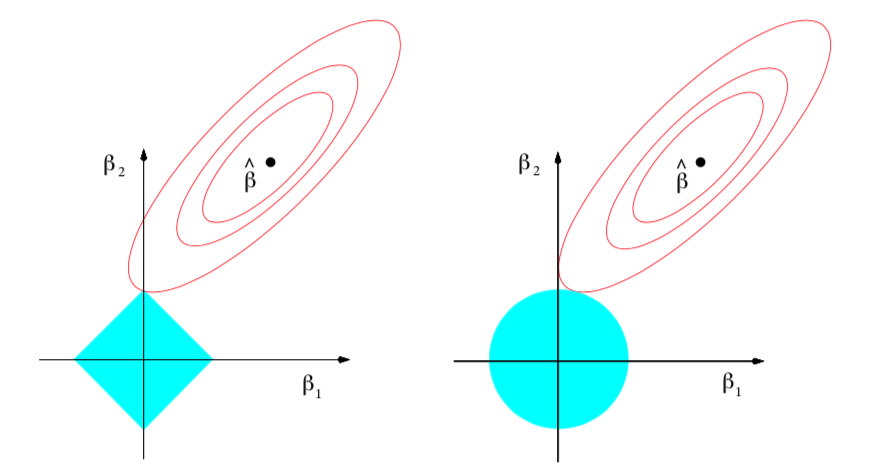
\includegraphics[scale=0.4]{img/ridge_lasso}
\caption{Constraints of Ridge and Lasso regressions.}
\label{ridge_lasso}
\end{figure}

Also other penalization factors can be chosen, \autoref{penalization}

\begin{figure}
\centering
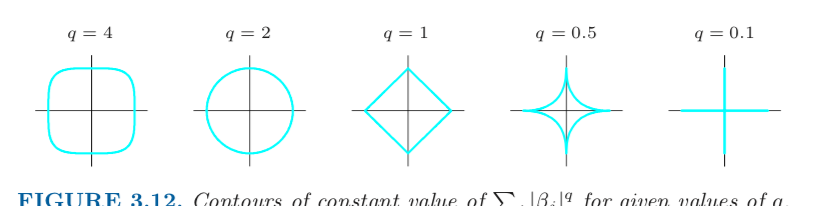
\includegraphics[scale=0.4]{img/penalization}
\caption{Shapes of different penalization factors.}
\label{penalization}
\end{figure}

\subsubsection{Least angle regression}
It is similar to forward stepwise. At first it identifies the variable most correlated with the response but instead of fitting it completely, it moves the variable toward its least squares value. As soon as another value gets correlated to the residual as the previous variable, the process is paused. The second variable joins the active set and their coefficients are moved together in a way that keeps their correlations tied and decreasing. The process is continued until all the variables are in the model.
\begin{algorithm}[!ht]
standardize the predictors to have $0$ mean and unit norm\;
$\mathcal{A}_k\leftarrow 0$\;
$r\leftarrow y-\bar{y}$, $\beta_i=0$ for $i\ne0$\;
\While {$|\mathcal{A}_k|<p$}{
find the predictor most correlated to $r$\;
insert the predictor in the active set $\mathcal{A}_k$\;

move the coefficients of the predictors in the active set to the direction defined by their joint least squares coefficient of the current residual, i.e.,
\begin{equation}
\delta_k = \left( X_{\mathcal{A}_k}^T X_{\mathcal{A}_k}\right)^{-1} X_{\mathcal{A}_k}^T r_k
\end{equation}
(where $\mathcal{A}_k$ is the current active set of variables) until some other competitor $x_\ell$ has as much correlation with the current residual\;
$r_k\leftarrow y - X_{\mathcal{A}_k}\beta_{\mathcal{A}_k}$
}
\end{algorithm}
After $min(N-1,p)$ steps we we arrive at the full least squares solution.
The coefficient profile evolves as
\begin{equation}
\beta_{\mathcal{A}_k} =  \beta_{\mathcal{A}_k} + \alpha \delta_k
\end{equation}

If to the LAR algorithm we add the following rule i.e.,

\textit{If a non-zero coefficient hits $0$, drop its variable from the active set of variables and recompute the current joint least squares direction.}

we get the same coefficient path of the lasso and this is called LAR(lasso). So this become an efficient solution to compute the Lasso problem, especially with $N>>p$ since Lasso can take more than $p$ steps while LAR require $p$ steps and it is efficient since it requires the same complexity as that of a single least squares fit using the $p$ predictors.

\subsection{Derived input directions methods}
When a large number of inputs is present, often there is a high correlation among them. In this case is convenient to regress on a new set inputs obtained form a linear combination of the original input.

\subsubsection{Principal component analysis}
The first input must be standardized since this analysis depends on the scaling. The principal components are defined as  	
\begin{equation}
z_i = X v_i
\end{equation}
where $v_i$ are the column vectors of $V$ from the SVD decomposition of $X=U\Sigma V^T$ (recall that $z_m$ are orthogonal)(\autoref{SVD}). The algorithm then regress $X$ on $z_1,\cdots, z_M$ for $M\le p$ and we have:

\begin{equation}
\hat{y}^{pcr}_{(M)} = \bar{y}\mathbf{1} + \sum_{m=1}^M \hat{\theta}_m z_m
\end{equation}
where $\hat{\theta}_m = \langle z_m, y\rangle/\langle z_m, z_m \rangle$. Since $z_m$ are linear combination of the original predictors $x_j$, we can express the solution as 

\begin{equation}
\hat{\beta}^{pcr}(M) = \sum_{m=1}^{M} \hat{\theta}_m v_m
\end{equation}
With $M=p$ we get the usual least squares. Principal component analysis discards the $p-M$ smallest eigenvalue components.

The value $M$ is suggested by cross-validation.

\begin{theorem}{\tb{PCA seeks principal directions of highest variance under the unit-norm constraint}}
\label{PCAmaxVar}
\begin{proof}
Consider an input space $\X$ endowed with the inner product operation $\langle \x_i, \x_j\rangle = \x_i^T \x_j$. Let $\{\x_1\}, \x_2, \cdots, \x_n$ denote a set of available data (observations) from $\X$. Let us call the axes that maximise the variance $\psi_1, \cdots, \psi_k$. Consider the first axis $\psi_1$ and project data onto it. The mean of the projection is $\langle \psi, \bar{x}\rangle$ with $\bar{x} = \frac{1}{N} \sum_{i=1}^n \x_i$.
By applying the variance definition:
\begin{equation}
\begin{aligned}
\sigma^2 &= \E\left[ \br{\psi_1^T\x -\E\left[ \psi^T\x\right]}^2 \right] = \\
&= \E\left[ \br{\psi_1^T\br{\x - \E\left[\x\right]}}^2 \right] = \\
&= \E\left[ \br{\psi_1^T\br{\x - \bar{\x}}}^2 \right] = \\
&= \E\left[ \psi_1^T\br{\x - \bar{\x}}^T\br{\x - \bar{\x}}\psi_1 \right] = \\
&= \psi_1^T\E\left[ \br{\x - \bar{\x}}^T\br{\x - \bar{\x}} \right]\psi_1  =\psi_1^T S \psi_1 
\end{aligned}
\end{equation}
where $S$ is the covariance matrix, i.e., the measure of the directional relationship between two random variables.
The variance must be maximized. A simple way would be to make $psi_1$ as big as possible but that is not an interesting solution. That is why is module is restricted: $\psi_1^T \psi_1=1$. To combine the objective and constraint the Lagrange multipliers are used:
\begin{equation}
\begin{aligned}
L &= \psi_1^T S \psi_1  - \alpha_1 \psi_1^T \psi -1\\
\Rightarrow \frac{\partial L}{\partial \psi_1} &= \cancel{2}S \psi -\cancel{2} \alpha_1 = 0\\
\Rightarrow \alpha_1 \psi_1 &= S \psi_1
\end{aligned}
\end{equation}
So the pair $\br{\alpha_1, \psi_1}$ is an eigenvalue-eigenvector pair. We can define additional principal components in an incremental fashion by choosing each new direction to be that which maximizes the projected variance amongst all possible directions orthogonal to those already considered (eigenvectors are not always perpendicular). In order to do so, one might consider to remove from the covariance matrix the component corresponding to the projection of the previously found axis and maximise the covariance of the residual. Suppose at step $\ell$ one found $\ell$ axis: then instead of using $S$ one will use: $S-[\psi_1, \cdots, \psi_\ell, 0, \cdots 0]^T S$.

These are the axes that maximize the variance. Recalling that PCA is obtained through SVD and recalling the property of SVD in \autoref{SVDEigenDec}, it is clear that PCA maximize the variance.
\end{proof}
\end{theorem}
Eigenvectors lie in the span of data and eigenvectors associated to the largest eigenvalues provides a low-dimensional subspace:

\begin{equation}
\begin{aligned}
\psi_\ell  &= \frac{1}{\lambda_\ell} S \psi_\ell = \frac{1}{\lambda_\ell} \br{\frac{1}{n}X^TX} \psi_\ell = \frac{1}{n\lambda_\ell} \left[\x_1, \cdots, \x_n \right] \begin{bmatrix} \x_1^T \\ \vdots\\ \x_n^T\end{bmatrix} \psi_\ell = \\
&= \frac{1}{n\lambda_\ell} \left[\begin{smallmatrix}
	x_{11}^2 +\cdots  +x_{n1}^2             & x_{11}x_{12}+\cdots +x_{n1}x_{n2}& \cdots &x_{11}x_{1k}+\cdots +x_{n1}x_{nk}\\
	x_{12} x_{11} +\cdots + x_{n2}x_{n1} & x_{12}^2+\cdots +x_{n2}^2          &\cdots &x_{12}x_{1k}+\cdots +x_{n2}x_{nk}\\
	\vdots&\vdots&\cdots &\vdots \\
	x_{1k} x_{11} +\cdots + x_{nk}x_{n1} & x_{1k}x_{12} +\cdots +x_{nk}x_{n2}  &\cdots &x_{1k}^2+\cdots +x_{nk}^2
\end{smallmatrix}\right]\psi_\ell =\\
&= \frac{1}{n\lambda_\ell} \begin{bmatrix}
\sum_{i=1}^n x_{i1}^2     &\sum_{i=1}^n x_{i1}x_{i2}& \cdots &\sum_{i=1}^n x_{i1}x_{ik}\\
\sum_{i=1}^nx_{i2} x_{i1} & \sum_{i=1}^n x_{i2}^2          &\cdots &\sum_{i=1}^n x_{i2}x_{ik}\\
\vdots&\vdots&\cdots &\vdots \\
\sum_{i=1}^n x_{ik} x_{i1}  & \sum_{i=1}^n x_{ik}x_{i2}         &\cdots &\sum_{i=1}^n x_{ik}^2
\end{bmatrix}\psi_\ell = \\
&=\sum_{i=1}^n \br{\x_i \x_i^T}\psi_\ell = \sum_{i=1}^n \br{\x_i \x_i^T\psi_\ell} = \sum_{i=1}^n \langle \x_i,\psi_\ell\rangle\x_i
\end{aligned}
\end{equation}

Principal components can be written as linear combinations of input data:
\begin{equation}
\label{PCALinComb}
\psi_\ell = \sum_{i=1}^n \alpha_{il} \x_i
\end{equation}

%the following has also another element
%\psi_\ell  &= \frac{1}{\lambda_\ell} S \psi_\ell = \frac{1}{\lambda_\ell} \br{\frac{1}{n}X^TX} \psi_\ell = \\
%&= \frac{1}{n\lambda_\ell} \left[\x_1, \cdots, \x_n \right] \begin{bmatrix} \x_1^T \\ \vdots\\ \x_n^T\end{bmatrix} \psi_\ell = \\
%&= \frac{1}{n\lambda_\ell} \begin{bmatrix}
%x_{11}^2 + x_{21}^2 +\cdots  +x_{n1}^2             & x_{11}x_{12}+x_{21}x_{22} +\cdots +x_{n1}x_{n2}&\cdots &x_{11}x_{1k}+x_{21}x_{2k} +\cdots +x_{n1}x_{nk}\\
%x_{12} x_{11} + x_{22}x_{21} +\cdots + x_{n2}x_{n1} & x_{12}^2+x_{22}^2 +\cdots +x_{n2}^2          &\cdots &x_{12}x_{1k}+x_{22}x_{2k} +\cdots +x_{n2}x_{nk}\\
%\vdots&\vdots&\cdots &\vdots \\
%x_{1k} x_{11} + x_{2k}x_{21} +\cdots + x_{nk}x_{n1} & x_{1k}x_{12}+x_{2k}x_{22} +\cdots +x_{nk}x_{n2}          &\cdots &x_{1k}^2+x_{2k}^2 +\cdots +x_{nk}^2

\subsubsection{Partial least squares}
This technique use a set of linear combinations of $y$ in addition to $X$ for the construction. It is not scale invariant so each $\x_j$ must be standardized.
\begin{algorithm}
standardize $x_j$ to $0$ mean and $1$ variance\;
$\hat{y}^{(0)}\leftarrow \bar{y}\mathbf{1}$\;
$x_j^{(0)} \leftarrow x_j$ \;
\For{$m=1,\cdots, p$}
{
    $z_m  = \sum_{j=1}^p \hat{\phi}_{mj} x_j^{(m-1)}$ where $\hat{\phi}_{mj} = \langle x_j^{(m-1)}, y\rangle$ \; 
    $\hat{\theta}_m = \frac{\langle z_m, y\rangle}{\langle z_m, z_m\rangle} $\;
    $\hat{y}^m = \hat{y}^{(m-1)} + \hat{\theta}_m z_m$\;
    orthogonalize each $x_j^{m-1}$ w.r.t. $z_m: x_j^{(m)} = x_j^{(m-1)} - \frac{\langle z_m, x_j^{(m-1)}\rangle}{\langle z_m, z_m\rangle} z_m$, $j=1,\cdots, p$\;
}
Output the sequence of fitted vectors $\{\hat{y}^m\}_1^p$. Since ${z_\ell}_1^m$ are linear in $x_j$, so is $\hat{y}^{(m)} = X \hat{\beta}^{pls}(m)$. These coefficients can be recovered from the sequence of PLS transformations.
\end{algorithm}

Since PLS use $y$ to construct its directions, its solution path is not linear in $y$. It seeks direction with high variance and high correlation with the response while PCR only with high variance.

\subsection{Multioutput shrinkage and selection}
To apply selection and shrinkage methods in the multiple output case, one could apply a univariate technique individually to each outcome or simultaneously to all outcomes, i.e., different $\lambda$ in Ridge or Lasso can be used for each output or the same value can be adopted.

\subsection{Other derived algorithms}
\subsubsection{Incremental forward stagewise}
\begin{algorithm}
$r\leftarrow y$ \;
$\beta_i =0$ for $i\ne 0$\;
find the (standardized) predictor $x_j$ most correlated with the residual \;
$\beta_j \leftarrow \beta_j + \delta_j$ where $\delta_j = \epsilon sign\left[\langle x_j, r \rangle\right]$ and $\epsilon >0$ small\;
$r\leftarrow r-\delta_j x_j$\;
Repeat the steps many times until the residuals are uncorrelated with the predictors.
\end{algorithm}

\subsubsection{The Dantzig selector}
$\cdots$

\subsubsection{The Grouped Lasso}
$\cdots$
